\chapter{Microservices}
\label{chapter:microservices}

\section{Characteristics, Benefits and Challenges}

Microservices is a software architecture style that consists of loosely coupled and fine-grained services. The services run in their own processes environments and use lightweight communication mechanisms for coordination. Together, the services can be used to provide functionality that is beyond the functionality they are capable of on their own. Microservices are built upon a similar design philosophy as the Unix operating system which consists of separate programs with specific functionality that can cooperate through a universal interface \cite{raymond2003art}. In the case of microservices, it is specialized and autonomous services that cooperate through network calls. This architecture of isolated services can offer numerous advantages such as: technology heterogeneity, resilience of the overall system, scaling of individual parts and component composability \cite{newman2015building}.
\\ \\
A system that consists of multiple collaborative services with well defined application programming interfaces opens up the possibility to use different technologies for each services. Tools, such as programming languages and databases, can be chosen based on the requirements of each service rather than the interoperability with other parts of the system. This benefit also reduces the risk associated with the adoption of new technologies within organizations. A clear definition of service boundaries makes it easier to identify where a particular problem lies in a complicated system. In the ideal case a failure to a single components does not cascade to the system of a system and cause it to stop working. Smaller isolated services offer the possibility of horizontal scaling as opposed to vertical scaling, which is often the only option for monolithic services. In many cases services can even be scaled on demand with accompanying potential for cost savings. Similar to programs in Unix, services can be made reusable for different functionality within a system in a microservices architecture. This kind of infrastructure can increase the flexibility of a system through the bundling of different reusable and re-composable services.
\\ \\
While microservices have some clear benefits they also introduce various challenges, most of which are associated with the operation of distributed systems \cite{deutsch2004eight}. Increased operational overhead and complexity in network interaction between services are some of the main challenges that microservices introduce. In able to successfully attain the benefits of microservices greater consideration has to be directed towards deployment, testing and monitoring than in the case of monolithic systems. System operators and application developers will also have to be aware of concepts such as distributed transaction, race conditions, message serialisation and the CAP theorem. Microservices are there for not the best option for all use cases and each system has to be evaluated on an individual bases. Empirical examples indicates that microservices architecture evolved as a solution for the operation of complex systems \cite{thones2015microservices, microservicesNetflix}. In the case of more straightforwards systems the potential benefits of microservices are not necessarily worth the increased operational and network complexity.

\section{Asynchronous Communication}

Chat applications are event-based by nature so they benefit most from system architecture than can handle asynchronous collaboration between different components. The two main challenges associated with asynchronous systems, from the perspective of microservices, are how events are emitted and how consumers are informed of emitted events \cite{newman2015building}. Messages brokers, a type of message oriented middleware, are typically used to solve those problems. Most brokers can handle subscriptions and the state of consumers allowing a loosely coupled system architecture. Among messaging patterns, suitable for asynchronous event-based communication, are publish/subscribe and push/pull.
\\
\begin{figure}[h!]
	\centering
	\subfigure[Publish-Subscribe]{\raisebox{15mm}{\label{fig:pub-sub}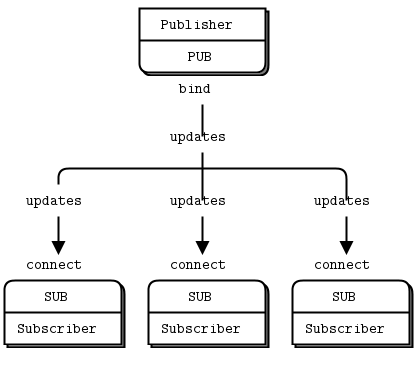
\includegraphics[width=0.45\textwidth]{images/pub-sub}}} \hfill
	\subfigure[Parallel Pipeline]{\label{fig:parallel-pipeline}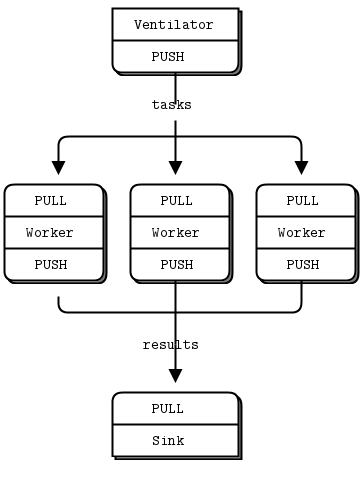
\includegraphics[width=0.45\textwidth]{images/parallel-pipeline}}
	\caption{Messaging patterns suitable for asynchronous communication \cite{hintjens2010zeromq}}
\end{figure}

\newpage
\noindent
The Publish/subscribe messaging pattern is used to distribute data from a single publisher to multiple receivers based on subscriptions as shown in Figure~\ref{fig:pub-sub}. For large systems the receivers are usually subscribed to a few available data sources only receive a fraction of all the published messages. Message brokers can take care of the filtering, to ensure that receivers only get messages they are subscribed to, and the actual routing of messages. Typical use cases for publish/subscribe include sending notifications asynchronously to multiple subscribers, like in a multi-user chat application.
\\ \\
The Push/pull messaging pattern, in the context of messaging brokers, can be seen as a pipelined form of publish/subscribe. It is used to distribute messages upon demand when a list of queued items need to be routed to a requester. A ventilator process push socket can be used to distribute tasks to workers and collect the result of their work from a push socket as shown in Figure~\ref{fig:parallel-pipeline}. This technique can be used for load-balancing and fair-share scheduling for a cluster of worker processes. A Use case for the push/pull messaging pattern is when a cluster of worker processes are used for multiple concurrent API calls.

\section{Containerized Virtualization}

A container is a virtualized runtime environment that runs as an application on a shared operating system. Containerized virtualization requires less overhead than hypervisor-based virtualization. The kernel and system libraries of the underlying operating system are shared and abstracted in the case of containers while the hypervisor abstracts the whole host machine in the case of virtual machines. This lightweightness makes it possible to run more containers than virtual machine on the same underlying hardware and possibly achieve better performance \cite{xavier2013performance}.
\\
\begin{figure}[h!]
	\subfigure[Standard virtualization]{\label{fig:standard-virtualization}
\includegraphics[width=0.45\textwidth]{images/standard-virtualization}} \hfill
	\subfigure[Container-based virtualization]{\raisebox{8mm}{\label{fig:containers}
\includegraphics[width=0.45\textwidth]{images/containers}}}
\caption{A comparison of standard virtualization and container-based virtualization}
\label{request-headers}
\end{figure}

\noindent
Apart from less overhead, the main benefit of containers is to increase the portability of applications. Containerized virtualization makes it possible to create portable production-like run-time environments that can be used during development. One of the main selling points of containerized virtualization is that deployment inside containers makes it possible to run the same application in multiple settings like physical servers, virtual machines and various cloud environments without requiring any additional adjustments. As with microservices, containers introduce a set of challenges such as the discovery of services, which the hypervisor usually takes care of in the case of virtual machines, and the fact that containers running on the same host are not completely isolated from each other. This requires a slightly different mindset, with regards to deployment, than in the case of standard virtualisation where each application environment is completely isolated.
\\ \\
Containers are a Linux-based technology provided by LXC (Linux Containers) or LXD (Linux Container Daemon), CGManager (Control Group Manager) and LXCFS (Userspace filesystem for LXC). The foundation of the container technology is meant to be distribution and vendor neutral to ensure flexibility and portability in future implementations of this virtualization technology \cite{linuxContainers}.


